% Metaphor: map. Two axes a reader can name, and every item placed by
% where it falls on both -- reach for it when the point is *how things
% compare*, not how they connect. A map with arrows on it is usually a
% pipeline that has not admitted it yet.
%
% Idiom: `matrix`. The rows and columns are the layout, so no cell needs
% a coordinate and re-wording a label cannot collide with its neighbour.
% Each cell holds a real `\node` with a name, which is what lets
% `python -m chitragupta.review figure` measure this picture at all.
% House palette (docs/TIKZ-STYLE.md). These five lines travel *inside*
% every figure that uses them -- not a shared file, not a preamble: the
% renderer injects only \usepackage{tikz}, and a thesis fragment is
% \input into a document that has never heard of this project.
\definecolor{cgInk}{HTML}{1A1A1A}
\definecolor{cgFlow}{HTML}{0072B2}
\definecolor{cgAccent}{HTML}{D55E00}
\definecolor{cgAlt}{HTML}{009E73}
\definecolor{cgAux}{HTML}{56B4E9}
\usetikzlibrary{matrix}
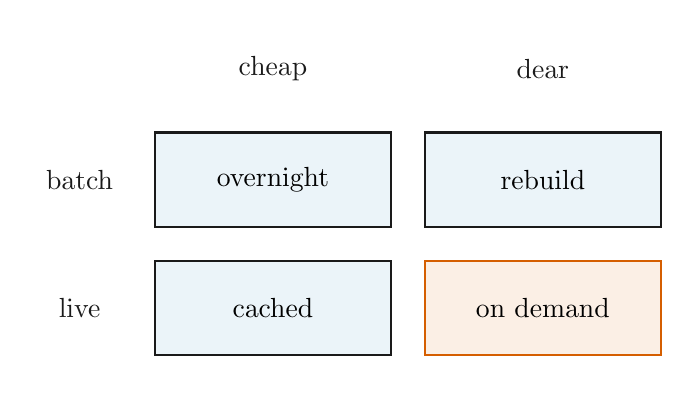
\begin{tikzpicture}[thick,
                    cell/.style={draw=cgInk,align=center,fill=cgFlow!8,
                                 minimum width=30mm,minimum height=12mm},
                    head/.style={align=center,minimum height=8mm,text=cgInk}]
  \matrix[row sep=4mm,column sep=4mm] {
    \node[head] (corner) {};        & \node[head] (cheap) {cheap};   & \node[head] (dear) {dear};    \\
    \node[head] (batch) {batch};    & \node[cell] (bc) {overnight};  & \node[cell] (bd) {rebuild};   \\
    \node[head] (live) {live};      & \node[cell] (lc) {cached};     & \node[cell,draw=cgAccent,fill=cgAccent!10] (ld) {on demand}; \\
  };
\end{tikzpicture}
